\documentclass[12pt,utf8,notheorems,compress,t]{beamer}
\usepackage{etex}

\usepackage[english]{babel}

\usepackage{mathtools}
\usepackage{booktabs}
\usepackage{array}
\usepackage{ragged2e}
\usepackage{multicol}
\usepackage{tabto}
\usepackage{xstring}
\usepackage{soul}\setul{0.3ex}{}
\usepackage[all]{xy}
\xyoption{rotate}
\usepackage{tikz}
\usetikzlibrary{calc,shapes.callouts,shapes.arrows,patterns}
\hypersetup{colorlinks=true}
\usepackage{multimedia}
\newcommand{\video}[2]{\movie[width=#2,height=#2,autostart,loop,poster]{}{#1}}
\hypersetup{colorlinks=false}

\usepackage{pifont}
\newcommand{\cmark}{\ding{51}}
\newcommand{\xmark}{\ding{55}}

\graphicspath{{images/}}

\usepackage[protrusion=true,expansion=true]{microtype}

\setlength\parskip{\medskipamount}
\setlength\parindent{0pt}

\title{Synthetic algebraic geometry and the phenomenon of nongeometric sequents}
\author{Ingo Blechschmidt}
\date{April 7th, 2018}

\useinnertheme[shadow=true]{rounded}
\useoutertheme{split}
\usecolortheme{orchid}
\usecolortheme{whale}
\setbeamerfont{block title}{size={}}

\useinnertheme{rectangles}

\usecolortheme{seahorse}
\definecolor{mypurple}{RGB}{150,0,255}
\setbeamercolor{structure}{fg=mypurple}
\definecolor{myred}{RGB}{150,0,0}
\setbeamercolor*{title}{bg=myred,fg=white}
\setbeamercolor*{titlelike}{bg=myred,fg=white}

\usefonttheme{serif}
\usepackage[T1]{fontenc}
\usepackage{libertine}

\newcommand{\A}{\mathcal{A}}
\renewcommand{\AA}{\mathbb{A}}
\newcommand{\E}{\mathcal{E}}
\newcommand{\F}{\mathcal{F}}
\renewcommand{\G}{\mathcal{G}}
\newcommand{\GG}{\mathbb{G}}
\renewcommand{\O}{\mathcal{O}}
\newcommand{\K}{\mathcal{K}}
\newcommand{\NN}{\mathbb{N}}
\newcommand{\RR}{\mathbb{R}}
\newcommand{\TT}{\mathbb{T}}
\newcommand{\PP}{\mathbb{P}}
\newcommand{\ZZ}{\mathbb{Z}}
\renewcommand{\P}{\mathcal{P}}
\newcommand{\ppp}{\mathfrak{p}}
\newcommand{\defeq}{\vcentcolon=}
\newcommand{\defeqv}{\vcentcolon\equiv}
\newcommand{\Sh}{\mathrm{Sh}}
\newcommand{\GL}{\mathrm{GL}}
\newcommand{\Zar}{\mathrm{Zar}}
\newcommand{\op}{\mathrm{op}}
\newcommand{\Set}{\mathrm{Set}}
\newcommand{\Eff}{\mathrm{Ef{}f}}
\newcommand{\Sch}{\mathrm{Sch}}
\newcommand{\Aff}{\mathrm{Aff}}
\newcommand{\LRS}{\mathrm{LRS}}
\newcommand{\Hom}{\mathrm{Hom}}
\newcommand{\Spec}{\mathrm{Spec}}
\newcommand{\lra}{\longrightarrow}
\newcommand{\RelSpec}{\operatorname{Spec}}
\renewcommand{\_}{\mathpunct{.}}
\newcommand{\?}{\,{:}\,}
\newcommand{\speak}[1]{\ulcorner\text{\textnormal{#1}}\urcorner}
\newcommand{\ull}[1]{\underline{#1}}
\newcommand{\affl}{\ensuremath{{\ull{\AA}^1}}}
\newcommand{\Ll}{\vcentcolon\!\Longleftrightarrow}
\newcommand{\inv}{inv.\@}
\newcommand{\seq}{\vdash_{\!\!\!\vec x}}

\setbeamertemplate{blocks}[rounded][shadow=false]

\newcommand{\fmini}[2]{\framebox{\begin{minipage}{#1}#2\end{minipage}}}
\makeatletter
\def\underunbrace#1{\mathop{\vtop{\m@th\ialign{##\crcr
      $\hfil\displaystyle{#1}\hfil$\crcr\noalign{\kern3\p@\nointerlineskip}
      \crcr\noalign{\kern3\p@}}}}\limits}
\def\overunbrace#1{\mathop{\vbox{\m@th\ialign{##\crcr\noalign{\kern3\p@}
      \crcr\noalign{\kern3\p@\nointerlineskip}
      $\hfil\displaystyle{#1}\hfil$\crcr}}}\limits}
\makeatother

\newenvironment{changemargin}[2]{%
  \begin{list}{}{%
    \setlength{\topsep}{0pt}%
    \setlength{\leftmargin}{#1}%
    \setlength{\rightmargin}{#2}%
    \setlength{\listparindent}{\parindent}%
    \setlength{\itemindent}{\parindent}%
    \setlength{\parsep}{\parskip}%
  }%
  \item[]}{\end{list}}

\newcommand{\pointthis}[2]{%
  \tikz[remember picture,baseline]{\node[anchor=base,inner sep=0,outer sep=0]%
    (#1) {#1};\node[overlay,rectangle callout,%
    callout relative pointer={(0.3cm,1.0cm)},fill=blue!20] at ($(#1.north)+(-0.1cm,-1.6cm)$) {#2};}%
}%

\newcommand{\hcancel}[5]{%
  \tikz[baseline=(tocancel.base)]{
    \node[inner sep=0pt,outer sep=0pt] (tocancel) {#1};
    \draw[red, line width=0.4mm] ($(tocancel.south west)+(#2,#3)$) -- ($(tocancel.north east)+(#4,#5)$);
  }%
}

\newcommand{\slogan}[1]{%
  \begin{center}%
    \setlength{\fboxrule}{2pt}%
    \setlength{\fboxsep}{8pt}%
    {\usebeamercolor[fg]{item}\fbox{\usebeamercolor[fg]{normal text}\parbox{0.93\textwidth}{#1}}}%
  \end{center}%
}

\newcommand{\sloganwithoutborder}[1]{%
  \begin{center}%
    \setlength{\fboxrule}{0pt}%
    \setlength{\fboxsep}{-14pt}%
    {\usebeamercolor[fg]{item}\fbox{\usebeamercolor[fg]{normal
    text}\parbox{0.9\textwidth}{\begin{center}#1\end{center}}}}%
  \end{center}%
}

% Adapted from https://latex.org/forum/viewtopic.php?t=2251 (Stefan Kottwitz)
\newenvironment<>{varblock}[2]{
  \begin{center}
    \begin{minipage}{#1}
      \setlength{\textwidth}{#1}
      \begin{actionenv}#3
	\def\insertblocktitle{\centering #2}
	\par
	\usebeamertemplate{block begin}}{
        \par
        \usebeamertemplate{block end}
      \end{actionenv}
    \end{minipage}
  \end{center}}

\setbeamertemplate{frametitle}{%
  \vskip0.7em%
  \leavevmode%
  \begin{beamercolorbox}[dp=1ex,center]{}%
      \usebeamercolor[fg]{item}{\textbf{{\Large \insertframetitle}}}
  \end{beamercolorbox}%
}

\setbeamertemplate{navigation symbols}{}

\newcounter{framenumberpreappendix}
\newcommand{\backupstart}{
  \setcounter{framenumberpreappendix}{\value{framenumber}}
}
\newcommand{\backupend}{
  \addtocounter{framenumberpreappendix}{-\value{framenumber}}
  \addtocounter{framenumber}{\value{framenumberpreappendix}} 
}

\setbeamertemplate{footline}{%
  \begin{beamercolorbox}[wd=\paperwidth,ht=2.25ex,dp=1ex,right,rightskip=1mm,leftskip=1mm]{}%
    \hfill
    \insertframenumber\,/\,\inserttotalframenumber
  \end{beamercolorbox}%
  \vskip0pt%
}


\newcommand{\hil}[1]{{\usebeamercolor[fg]{item}{\textbf{#1}}}}

\IfSubStr{\jobname}{\detokenize{nonotes}}{
  \setbeameroption{hide notes}
}{
  \setbeameroption{show notes}
}
\setbeamertemplate{note page}[plain]
\setbeameroption{hide notes}

\begin{document}

\addtocounter{framenumber}{-1}

\begin{frame}[c]
  \centering
  \medskip
  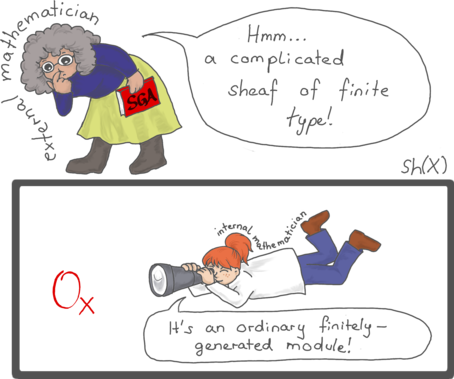
\includegraphics[scale=0.3]{images/external-internal-small}
  \medskip

  \hil{Synthetic algebraic geometry} \\
  \small\emph{a case study in applied topos theory}

  \large\&

  \normalsize

  \hil{the phenomenon of nongeometric sequents}

  \medskip

  \scriptsize
  Ingo Blechschmidt \\
  University of Augsburg
  \medskip

  103rd Peripatetic Seminar on Sheaves and Logic in Brno \\
  April 7th, 2018
  \par
\end{frame}


\section{Preliminaries}

\subsection{Approaches to algebraic geometry}

\begin{frame}{Approaches to algebraic geometry}
  Usual approach to algebraic geometry: \hil{layer schemes above ordinary set theory}
  using either
  \begin{itemize}
    \item locally ringed spaces
    \small
    \begin{multline*}
      \text{set of prime ideals of~$\ZZ[X,Y,Z]/(X^n+Y^n-Z^n)$} + {} \\
      \text{Zariski topology} + \text{structure sheaf}
    \end{multline*}
    \normalsize
    \item or Grothendieck's functor-of-points account, where a scheme is a functor~$\mathrm{Ring} \to \mathrm{Set}$.
    \small\[ A \longmapsto \{ (x,y,z) \in A^3 \,|\, x^n+y^n-z^n=0 \} \]
  \end{itemize}
  \bigskip

  \hil{Synthetic approach:} model schemes \hil{directly as sets} in a certain
  nonclassical set theory.
  \small
  \[ \{ (x,y,z) \? (\affl)^3 \,|\, x^n+y^n-z^n=0 \} \]
\end{frame}


\subsection{Toposes as universes}

\begin{frame}{Toposes as mathematical universes}
  A \hil{topos} is a category which has finite limits,
  is cartesian closed and has a subobject classifier, for instance
  \begin{itemize}
    \item \hil{$\boldsymbol{\Set}$}, the category of sets;
    \item \hil{$\boldsymbol{\Sh(X)}$}, the category of set-valued sheaves over
    a space~$X$;
    \item \hil{$\boldsymbol{\Eff}$}, the ef{}fective topos (roughly: a
    category of data types).
  \end{itemize}

  \begin{varblock}{9cm}{}Any topos supports an \hil{internal language},
  which is sound with respect to
  \only<1>{\hil{intuitionistic reasoning}}%
  \only<2->{\hil{\pointthis{intuitionistic reasoning}{
    \textnormal{\textcolor{black}{
    no $\varphi \vee \neg\varphi$,\ \
    no $\neg\neg\varphi \Rightarrow \varphi$,\ \
    no axiom of choice}}}}}.\end{varblock}
\end{frame}

\newcommand{\intex}[3]{#1 \quad #2\par #3\bigskip\medskip}

\begin{frame}{Curious universes}
  \begin{changemargin}{-1.1em}{0em}
    \small
    \begin{itemize}
      \item \intex{
        $\Eff \models \text{``There are infinitely many prime numbers.''}$
      }{\textcolor{green!90}{\cmark}}{
        External meaning: There is a \hil{Turing machine} producing arbitrarily many prime
        numbers.
      }

      \item \intex{
        $\Eff \models \text{``Any Turing machine halts or doesn't halt.''}$
      }{\textcolor{red!80}{\xmark}}{
        External meaning: There is a \hil{halting oracle} which determines whether
        any given machine halts or doesn't halt.
      }

      \item \intex{
        $\Sh(X) \models \text{``Any cont. function with opposite signs has
        a zero.''}$
      }{\textcolor{red!80}{\xmark}}{
        External meaning: Zeros can locally be picked \hil{continuously} in
        continuous families of continuous functions.
      }
    \end{itemize}
  \end{changemargin}

  \vspace*{-2em}
  \hfill\video{zeros-in-families.mp4}{2cm}
\end{frame}

\begin{frame}{Synthetic differential geometry}
  \vspace*{-1em}
  \begin{varblock}{9.5cm}{The axiom of microaffinity}
    \justifying
    Let~$\Delta = \{ \varepsilon \in \RR \,|\, \varepsilon^2 = 0 \}$.
    For any function $f : \Delta \to \RR$,
    there are unique numbers~$a, b \in \RR$ such that
    $f(\varepsilon) = a + b \varepsilon$
    for all~$\varepsilon \in \Delta$.
  \end{varblock}

  \begin{center}
    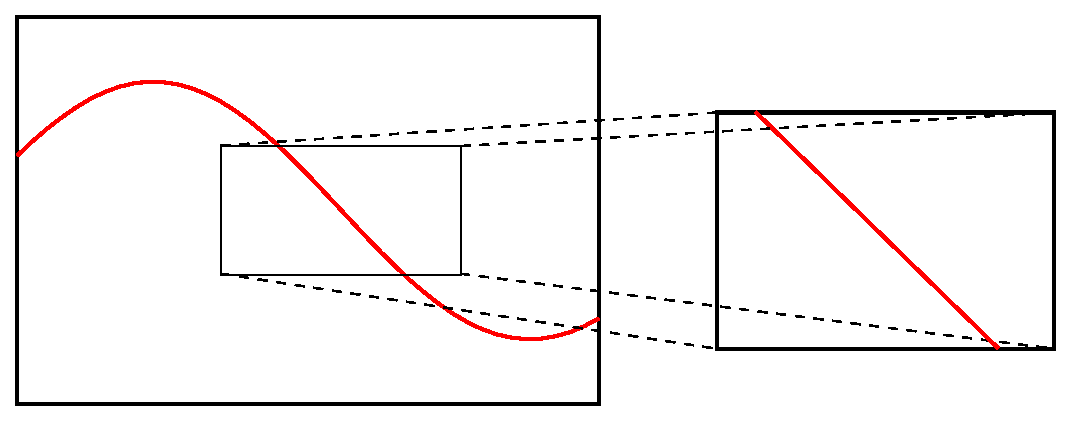
\includegraphics[width=0.5\textwidth]{microaffinity}
  \end{center}

  \vspace*{-1em}
  \begin{itemize}
    \item The \hil{derivative} of~$f$ as above at zero is~$b$.
    \item Manifolds are \hil{just sets}.
    \item A \hil{tangent vector} to~$M$ is a map~$\Delta \to M$.
  \end{itemize}

  \centering
  \hil{Toposes provide models for this theory.}
\end{frame}


\section{Synthetic algebraic geometry}


\subsection{The big Zariski topos}

\begin{frame}{The big Zariski topos}
  Let~$S$ be a fixed base scheme.

  \begin{block}{\centering Definition}\small
  The \hil{big Zariski topos} $\Zar(S)$ is the
  category $\Sh(\Sch/S)$. It consists of functors
  $(\Sch/S)^\op \to \Set$ satisfying the gluing condition that
  \[ F(T) \to
    \prod_i F(U_i) \rightrightarrows
    \prod_{j,k} F(U_j \cap U_k) \]
  \\[-0.6em]
  is a limit diagram for any scheme~$T = \bigcup_i U_i$ over~$S$.
  \end{block}

  \begin{changemargin}{-1.0em}{-0.5em}
  \begin{itemize}
    \item For an~$S$-scheme~$X$, its functor of points $\ull{X} =
    \Hom_S(\cdot,X)$ is an object of~$\Zar(S)$. It feels like \hil{the set of
    points} of~$X$. \\[0.2em]
    \item \ \\[-1.2em]\mbox{In particular, there is the ring object $\affl$ with~$\affl(T) =
    \O_T(T)$.} \\[0.2em]
    \item $\Zar(S)$ classifies local~$\O_S$-algebras which are local
    over~$\O_S$.
  \end{itemize}
  \end{changemargin}
\end{frame}


\subsection{Synthetic constructions}

\begin{frame}{Synthetic constructions}
  \small
  $\hil{$\boldsymbol{\mathbb{A}^n}$} = (\affl)^n = \affl \times \cdots \times \affl$

  $\begin{array}{@{}r@{}c@{}l@{}}
    \hil{$\boldsymbol{\mathbb{P}^n}$} &\phantom{}=\phantom{}& \{ (x_0,\ldots,x_n) : (\affl)^{n+1} \,|\, x_0 \neq 0 \vee
    \cdots \vee x_n \neq 0 \}/(\affl)^\times \\
    &\cong& \text{set of one-dimensional subspaces of~$(\affl)^{n+1}$} \\
    &&\qquad \text{(with~$\O(-1) = (\ell)_{\ell \? \mathbb{P}^n}$, $\O(1) =
    (\ell^\vee)_{\ell \? \mathbb{P}^n}$)}
  \end{array}$

  $\hil{$\boldsymbol{\Spec(R)}$} = \Hom_{\mathrm{Alg}(\affl)}(R, \affl) =
    \text{set of $\affl$-valued points of $R$}$

  $\hil{$\boldsymbol{TX}$} = X^\Delta$, where $\Delta = \{ \varepsilon \? \affl \,|\, \varepsilon^2 = 0 \}$

  A subset $U \subseteq X$ is \hil{qc-open} if and only if for any $x : X$
  there exist $f_1,\ldots,f_n \? \affl$ such that $x \in U \Longleftrightarrow
  \exists i\_ f_i \neq 0$.

  A \hil{synthetic affine scheme} is a set which is in bijection
  with~$\Spec(R)$ for some finitely presented algebra~$R$.

  A \hil{synthetic scheme} is a set which can be covered by finitely many
  qc-open synthetic affine schemes~$U_i$ such that the intersections~$U_i \cap
  U_j$ can be covered by finitely many qc-open synthetic affine schemes.
\end{frame}


\subsection[Quasicoherence]{Synthetic quasicoherence}

\begin{frame}{Properties of the affine line}
  \begin{itemize}
    \item $\affl$ is a local ring:
    \[ 1 \neq 0 \qquad\qquad \text{$x + y$ \inv} \Longrightarrow \text{$x$ \inv} \vee
    \text{$y$ \inv} \]
    \item $\affl$ is a field:
    \begin{align*}
      \neg(x = 0) &\Longleftrightarrow \text{$x$ invertible} \\
      \neg(\text{$x$ invertible}) &\Longleftrightarrow \text{$x$ nilpotent}
    \end{align*}
    \item $\affl$ satisfies the axiom of microaffinity: Any map $f : \Delta \to
    \affl$ is of the form~$f(\varepsilon) = a + b \varepsilon$ for unique
    values~$a,b \? \affl$, where~$\Delta = \{ \varepsilon \? \affl \,|\,
    \varepsilon^2 = 0 \}$.
    \item Any function $\affl \to \affl$ is a polynomial.
    \item $\affl$ is anonymously algebraically closed: Any monic polynomial
    does \emph{not not} have a zero.
    \item $\affl$ is of unbounded Krull dimension.
  \end{itemize}
\end{frame}

\begin{frame}{Synthetic quasicoherence}
  Recall~$\Spec(R) = \Hom_{\mathrm{Alg}(\affl)}(R, \affl)$ and consider the statement
  \[ \text{``the canonical map~$
    \begin{array}[t]{rcl}
      R &\longrightarrow& (\affl)^{\Spec(R)} \\
      f &\longmapsto& (\alpha \mapsto \alpha(f))
    \end{array}
  $ is bijective''}.
  \]
  \vspace*{-1em}

  \begin{itemize}
    \item True for~$R = \affl[X]/(X^2)$ (microaffinity).
    \item True for~$R = \affl[X]$ (every function is a polynomial).
    \item True for \hil{any} finitely presented~$\affl$-algebra~$R$.
  \end{itemize}

  Any known property of~$\affl$ follows from this \hil{synthetic
  quasicoherence}.

  \emph{Example.} Let~$x \? \affl$ such that~$x \neq 0$. Set~$R = \affl/(x)$.
  Then~$\Spec(R) = \emptyset$. Thus~$(\affl)^{\Spec(R)}$ is a singleton.
  Hence~$R = 0$. Therefore~$x$ is invertible.
\end{frame}


\section{Nongeometric sequents}

\begin{frame}{Nongeometric sequents}
  \small
  Let~$\TT$ be a \hil{geometric theory} (rings, intervals, \ldots).

  \vspace*{-2em}
  \begin{varblock}{11cm}{}  %Fundamental theorem about classifying toposes}
    For a \hil{geometric sequent}~$\forall \vec x\_ (\varphi \Rightarrow \psi)$, the following
    are equivalent:
    \begin{enumerate}
      \item It is \hil{provable} by~$\TT$. \\[-1em]
      \item It holds
      \hil{for all models} of~$\TT$ in all toposes. \\[-1em]
      \item It holds
      for the \hil{generic model} of~$\TT$ in its \hil{classifying topos}.
    \end{enumerate}
  \end{varblock}

  \begin{itemize}
    \item Additional \hil{nongeometric sequents} may hold in a classifying
    topos, for instance~``$\affl$ is synthetically quasicoherent''
    in~$\Zar(S)$. \\[-1em]
    \item These are \hil{$\boldsymbol{\TT}$-redundant}, but the converse is
    false. \\[-1em]  % (Bezem--Buchholtz--Coquand 2017). \\[-1em]
    \item \ \\[-1.2em]\mbox{Are they precisely the consequences of synthetic
    quasicoherence?} \\[-1em]
    \item Applications: synthetic algebraic geometry,
    generic freeness, \ldots
  \end{itemize}
\end{frame}


\section{Further research}

\begin{frame}{Further research}
  \vspace*{-1em}
  \small
  \begin{itemize}
    \item Push synthetic algebraic geometry further:
          true cohomology, intersection theory, derived categories, \ldots
          \\[-1.9em]

    \item What do the various subtoposes of~$\Zar(S)$ classify
          (étale, fppf, ph, $\neg\neg$, \ldots)? What about the crystalline
          topos?
          \\[-1.9em]

    \item Understand quasicoherence.
          \\[-1.9em]

    \item Find further applications of nongeometric sequents, for instance in
    constructive algebra.
  \end{itemize}

  {\vspace{-0.1em}\centering
  \rotatebox{90}{\tiny\scalebox{0.5}{Illustration: Carina Willbold}}\hspace{-0.05cm}%
  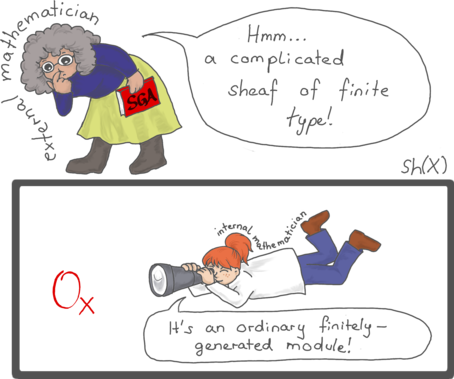
\includegraphics[scale=0.18]{images/external-internal-small}
  \par\medskip\vspace{-0.5em}}

  \centering
  Expository notes: \\
  \hil{\href{https://www.ingo-blechschmidt.eu/}{https://www.ingo-blechschmidt.eu/}}
  \par
\end{frame}

\addtocounter{framenumber}{-1}

\end{document}



"Any map from the reals to the reals is smooth." This statement holds in the
context of synthetic differential geometry, a well-developed account of smooth
manifolds and related notions which allows us to bring formal reasoning much
closer to geometric intuition.

We employ the internal language of the big Zariski topos of a base scheme to
give a similar account of algebraic geometry, reminiscent of the language of
the classical Italian school and incorporating Grothendieck's functor-of-points
philosophy. From the point of view of the Zariski topos, a scheme over the base
will look like a plain old set, and the affine line will look like a certain
field. Central to the synthetic account is the notion of "synthetic
quasicoherence", which doesn't have an analog in synthetic differential
geometry and which gives the account a distinct algebraic flavor.

The higher-order axiom of synthetic quasicoherence implies all known internal
properties of the affine line, for instance that it is a field and that it is
algebraically closed in a weak sense. We surmise that this is for a deeper
reason, related to the age-old question "which nongeometric sequents hold in
the classifying topos of a geometric theory?". The second part of the talk
reports on work in progress about this topic.
